% Unit 1 guided notes -- 5 block lessons.
% Single source: student + key, print + LMS, selected via build toggles.
\documentclass{apchem-notes}

\apcunit{1}
\apcunittitle{Atomic Structure and Properties}
\apcdoctitle{Guided Notes}
\apcsubtitle{CED 1.1--1.8 \textbullet\ Zumdahl \S3.2--3.7, \S7.5--7.12, \S8.4}

\begin{document}
\apctitleblock

% =====================================================================
\blocklesson{Moles and Mass Spectra}{Wed Aug 12}

\begin{objectives}
  \item Convert among grams, moles, and particles using molar mass and
        Avogadro's number.
  \item Compute an average atomic mass from a mass spectrum and identify
        the element.
\end{objectives}

\reading{Zumdahl \S3.2--3.5}{112--123}

\begin{warmup}[3]
  \item Express \num{0.00520} in scientific notation:
        \answerblank[3cm]{$5.20\times10^{-3}$}
  \item How many significant figures in \SI{100.0}{\gram}?
        \answerblank[2cm]{4}
  \item Name \ce{MgCl2}: \answerblank[4cm]{magnesium chloride}
\end{warmup}

\segment{INSTRUCTION A}{25}{The mole: chemistry's counting unit}

\notesection{Why count by weighing}{1.1}
\practice{5}

Atoms are too small to count directly, so we count them the way a bank counts
coins: \term{by weighing}. The bridge between mass and count is the
\term{mole}:
\[
  \answerblank[5.5cm]{1 mol $= 6.022\times10^{23}$ particles}
  \qquad\text{(Avogadro's number, } N_A\text{)}
\]

\notesub{Molar mass}

The \term{molar mass} $M$ (\si{\gram\per\mole}) is numerically equal to the
average atomic mass on the periodic table. For a compound, add the atoms:

\ce{CaCO3}: \quad $M = 40.08 + 12.01 + 3(16.00) =$
\answerblank[3cm]{\SI{100.09}{\gram\per\mole}}

\notesub{The mole road map}

\begin{center}
\begin{tikzpicture}[node distance=3.2cm, font=\sffamily\small]
  \node[draw=apcaccent, thick, rounded corners, minimum height=0.9cm] (g) {grams};
  \node[draw=apcaccent, thick, rounded corners, minimum height=0.9cm, right=of g] (mol) {moles};
  \node[draw=apcaccent, thick, rounded corners, minimum height=0.9cm, right=of mol] (p) {particles};
  \draw[-{Stealth}, thick] (g.north east) to[bend left=20]
    node[above]{$\div\,M$} (mol.north west);
  \draw[-{Stealth}, thick] (mol.south west) to[bend left=20]
    node[below]{$\times\,M$} (g.south east);
  \draw[-{Stealth}, thick] (mol.north east) to[bend left=20]
    node[above]{$\times\,N_A$} (p.north west);
  \draw[-{Stealth}, thick] (p.south west) to[bend left=20]
    node[below]{$\div\,N_A$} (mol.south east);
\end{tikzpicture}
\end{center}

\begin{apcnote}
Every path runs \emph{through moles}. There is no direct road from grams to
particles --- that shortcut is where setups go wrong.
\end{apcnote}

\begin{workedexample}[Worked example: three-step conversion]
How many oxygen \emph{atoms} are in \SI{10.0}{\gram} of \ce{CaCO3}?
\begin{align*}
  n &= \frac{\SI{10.0}{\gram}}{\SI{100.09}{\gram\per\mole}}
     = \SI{9.99e-2}{\mole}\ \ce{CaCO3}\\
  N &= (9.99\times10^{-2})(6.022\times10^{23})
     = 6.02\times10^{22}\ \text{formula units}\\
  N_{\ce{O}} &= 3 \times 6.02\times10^{22} = 1.80\times10^{23}\ \text{O atoms}
\end{align*}
\end{workedexample}

\segment{GUIDED PRACTICE}{15}{Mole conversions --- you drive}

\begin{enumerate}[leftmargin=*,itemsep=0.4em]
  \item Moles in \SI{4.50}{\gram} of \ce{H2O}:
        \answerblank[3.5cm]{\SI{0.250}{\mole}}
  \item Mass of \SI{0.30}{\mole} of \ce{NaCl}:
        \answerblank[3.5cm]{\SI{17.5}{\gram} ($\approx$ 18 g)}
  \item Molecules in \SI{0.25}{\mole} of \ce{CO2}:
        \answerblank[3.5cm]{$1.5\times10^{23}$}
  \item Hydrogen atoms in \SI{1.0}{\mole} of \ce{NH3}:
        \answerblank[3.5cm]{$1.8\times10^{24}$}
\end{enumerate}

\segment{INSTRUCTION B}{20}{Mass spectra: where atomic masses come from}

\notesection{Isotopes and average atomic mass}{1.2}
\practice{4}

Most elements are mixtures of \term{isotopes} --- same protons, different
\answerblank[2.5cm]{neutrons}. The periodic-table mass is a
\term{weighted average}:
\[
  \bar{m} = \answerblank[5cm]{$\sum(\text{abundance} \times \text{mass})$}
\]

\notesub{Reading a mass spectrum}

A \term{mass spectrometer} vaporizes and ionizes a sample, then sorts ions by
mass. On the spectrum:
\begin{itemize}[leftmargin=*, itemsep=0.15em]
  \item peak \term{position} (x-axis) $\to$ \answerblank[4cm]{isotope mass}
  \item peak \term{height/area} (y-axis) $\to$ \answerblank[4cm]{relative abundance}
  \item number of peaks $\to$ \answerblank[4cm]{number of isotopes}
\end{itemize}

\begin{workedexample}[Worked example: magnesium]
A magnesium spectrum shows peaks at 24 u (79\%), 25 u (10\%), and 26 u (11\%).
\[
  \bar{m} = 0.79(24) + 0.10(25) + 0.11(26) = \SI{24.3}{u}
\]
The average sits \emph{near 24} because \ce{^{24}Mg} dominates --- a weighted
average always leans toward the most abundant isotope.
\end{workedexample}

\begin{apctrap}
``Average the peak masses'' --- $(24+25+26)/3 = 25$ --- ignores abundance and
is the single most common Unit 1 error. The AP answer requires the
\emph{weighted} setup even when the arithmetic is easy.
\end{apctrap}

\segment{APPLICATION}{20}{Spectrum interpretation}

An element's spectrum shows exactly two peaks: 69 u (60.1\%) and 71 u (39.9\%).

\begin{enumerate}[leftmargin=*,itemsep=0.4em]
  \item Estimate the average atomic mass \emph{before computing}: closer to 69
        or 71? Why?
        \answerlines[2]{Closer to 69 --- the 69 u isotope is more abundant, so
        the weighted average leans toward it.}
  \item Compute it. \workspace[2.2cm]
        \keyonly{\begin{apcanswer}$0.601(69)+0.399(71)=\SI{69.8}{u}$ --- gallium.\end{apcanswer}}
  \item A student claims the sample must contain two different elements
        because there are two peaks. Refute in one sentence.
        \answerlines[2]{Both peaks have the same proton count --- they are
        isotopes of one element differing only in neutrons.}
\end{enumerate}

\begin{exitticket}
Boron: \ce{^{10}B} 19.9\%, \ce{^{11}B} 80.1\%. Estimate the average atomic
mass to one decimal and justify the direction it leans.
\answerlines[2]{$0.199(10.0)+0.801(11.0)=\SI{10.8}{u}$; leans toward 11
because \ce{^{11}B} dominates.}
\end{exitticket}

% =====================================================================
\blocklesson{Formulas from Data}{Fri Aug 14}

\begin{objectives}
  \item Compute percent composition from a formula, and a formula from
        percent composition.
  \item Distinguish empirical from molecular formulas and connect them via
        molar mass.
  \item Classify matter as pure substance or mixture from particulate
        diagrams.
\end{objectives}

\reading{Zumdahl \S3.6--3.7}{123--132}\quad\reading{\S1.10}{53--57}

\begin{warmup}[3]
  \item Molar mass of \ce{CO2}: \answerblank[3cm]{\SI{44.01}{\gram\per\mole}}
  \item Moles in \SI{9.0}{\gram} \ce{H2O}: \answerblank[3cm]{\SI{0.50}{\mole}}
  \item Mass spectrum peaks at 63 u and 65 u, heights 7 : 3. Which isotope is
        more abundant? \answerblank[3cm]{\ce{^{63}Cu} (63 u)}
\end{warmup}

\segment{INSTRUCTION A}{25}{Percent composition and empirical formulas}

\notesection{Percent composition}{1.3}
\practice{5}

\[
  \%\,\text{element} =
  \answerblank[6.6cm]{$\dfrac{\text{mass of element in 1 mol}}{\text{molar mass}}\times 100\%$}
\]

\ce{H2O}: \quad $\%\,\ce{O} = \dfrac{16.00}{18.02}\times100\% =$
\answerblank[2.5cm]{88.8\%}

\notesub{From percent to formula: the four-step recipe}

\begin{enumerate}[leftmargin=*,itemsep=0.2em]
  \item Assume a \answerblank[3cm]{100 g} sample $\to$ percents become grams.
  \item Convert each element to \answerblank[2.5cm]{moles}.
  \item Divide every mole value by the \answerblank[3cm]{smallest} of them.
  \item If ratios aren't whole, multiply all by a small integer
        (\,.5\,$\to\times2$,\ \ .33\,$\to\times3$\,).
\end{enumerate}

\begin{workedexample}[Worked example: vitamin C]
40.9\% C, 4.58\% H, 54.5\% O; molar mass $\approx \SI{176}{\gram\per\mole}$.
\begin{align*}
  \ce{C}&: 40.9/12.01 = 3.41 & \ce{H}&: 4.58/1.008 = 4.54 & \ce{O}&: 54.5/16.00 = 3.41\\
  \ce{C}&: 3.41/3.41 = 1     & \ce{H}&: 4.54/3.41 = 1.33  & \ce{O}&: 3.41/3.41 = 1
\end{align*}
$\times 3$: empirical \ce{C3H4O3} ($M_{emp}=88.06$).
Since $176/88.06 = 2$, molecular formula = \ce{C6H8O6}.
\end{workedexample}

\begin{apctrap}
Never round 1.33 to 1. Ratios ending in .25, .33, .5, .67, .75 are signals to
multiply, not round. Rounding is only for values within $\sim$0.05 of a whole
number.
\end{apctrap}

\segment{GUIDED PRACTICE}{15}{Formula determination}

A compound is 75.0\% C and 25.0\% H by mass.

\begin{enumerate}[leftmargin=*,itemsep=0.4em]
  \item Empirical formula: \workspace[2cm]
        \keyonly{\begin{apcanswer}C: $75/12.01=6.25$; H: $25/1.008=24.8$;
        ratio $1:3.97 \to$ \ce{CH4}\end{apcanswer}}
  \item If the molar mass is \SI{16}{\gram\per\mole}, the molecular formula is
        \answerblank[2.5cm]{\ce{CH4}} --- empirical and molecular can be the
        \answerblank[2.5cm]{same}.
\end{enumerate}

\segment{INSTRUCTION B}{20}{Pure substances, mixtures, and hydrates}

\notesection{Classifying matter at the particle level}{1.4}
\practice{1}

\begin{center}
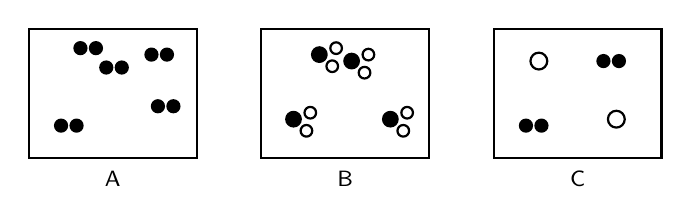
\begin{tikzpicture}[scale=0.82, font=\sffamily\footnotesize]
  % element
  \draw[thick] (0,0) rectangle (2.6,2);
  \foreach \x/\y in {0.5/0.5, 1.2/1.4, 2.0/0.8, 0.8/1.7, 1.9/1.6}
    {\fill[black] (\x,\y) circle (0.11) ++(0.24,0) circle (0.11);
     \draw (\x,\y) ++(0.12,0) circle (0pt);}
  \node[below] at (1.3,-0.05) {A};
  % compound
  \begin{scope}[xshift=3.6cm]
  \draw[thick] (0,0) rectangle (2.6,2);
  \foreach \x/\y in {0.5/0.6, 1.4/1.5, 2.0/0.6, 0.9/1.6}
    {\fill[black] (\x,\y) circle (0.13);
     \draw[thick] (\x,\y) ++(0.26,0.1) circle (0.09);
     \draw[thick] (\x,\y) ++(0.2,-0.18) circle (0.09);}
  \node[below] at (1.3,-0.05) {B};
  \end{scope}
  % mixture
  \begin{scope}[xshift=7.2cm]
  \draw[thick] (0,0) rectangle (2.6,2);
  \foreach \x/\y in {0.5/0.5, 1.7/1.5}
    {\fill[black] (\x,\y) circle (0.11) ++(0.24,0) circle (0.11);}
  \foreach \x/\y in {1.9/0.6, 0.7/1.5}
    {\draw[thick] (\x,\y) circle (0.13);}
  \node[below] at (1.3,-0.05) {C};
  \end{scope}
\end{tikzpicture}
\end{center}

Diagram A shows a pure \answerblank[2.6cm]{element} (diatomic);
B shows a pure \answerblank[2.8cm]{compound};
C shows a \answerblank[2.6cm]{mixture}.
The test: a pure substance has \answerblank[5.0cm]{only one kind of particle}.

\notesub{Mixtures have variable composition}

For a mixture, composition is a \emph{measured} quantity, not a formula.
A \SI{5.0}{\gram} mixture containing \SI{2.0}{\gram} \ce{NaCl} is
\answerblank[2.5cm]{40\%} \ce{NaCl} by mass.

\segment{APPLICATION}{20}{Hydrate analysis}

\ce{MgSO4 . 7 H2O} (Epsom salt) is a compound --- water molecules sit in fixed
ratio inside the crystal.

\begin{enumerate}[leftmargin=*,itemsep=0.4em]
  \item Molar mass of \ce{MgSO4 . 7 H2O}: \workspace[1.8cm]
        \keyonly{\begin{apcanswer}$120.4 + 7(18.02) = \SI{246.5}{\gram\per\mole}$\end{apcanswer}}
  \item Percent water by mass: \workspace[1.8cm]
        \keyonly{\begin{apcanswer}$126.1/246.5 \times 100\% = 51.2\%$\end{apcanswer}}
  \item Heating drives off the water. Is the white powder left behind the same
        substance you started with? Justify at the particle level.
        \answerlines[2]{No --- anhydrous \ce{MgSO4} has a different fixed
        composition (no water molecules in the lattice); a chemical change
        separated the hydrate into two substances.}
\end{enumerate}

\begin{exitticket}
A compound is 50.0\% S and 50.0\% O by mass. Find its empirical formula.
\answerlines[2]{S: $50/32.07=1.56$; O: $50/16.00=3.13$; ratio $1:2 \to$ \ce{SO2}}
\end{exitticket}

% =====================================================================
\blocklesson{Electron Configurations and Coulomb's Law}{Mon Aug 17}

\begin{objectives}
  \item Write ground-state configurations for atoms and ions; recognize
        excited states.
  \item Use Coulomb's law, shielding, and effective nuclear charge to compare
        electron energies.
\end{objectives}

\reading{Zumdahl \S7.5, 7.8--7.11}{346--364}

\begin{warmup}[4]
  \item Average mass from peaks 6 u (7.6\%) and 7 u (92.4\%):
        \answerblank[3cm]{\SI{6.9}{u} (Li)}
  \item Empirical formula of \ce{C6H12O6}: \answerblank[2.5cm]{\ce{CH2O}}
  \item Moles of \ce{O} atoms in \SI{0.50}{\mole} \ce{CO2}:
        \answerblank[2.5cm]{\SI{1.0}{\mole}}
  \item Protons / neutrons in \ce{^{37}Cl}: \answerblank[2.5cm]{17 / 20}
\end{warmup}

\segment{INSTRUCTION A}{25}{Where electrons live}

\notesection{Shells, subshells, and the filling order}{1.5}
\practice{1}

Electrons occupy \term{shells} ($n = 1, 2, 3\ldots$) divided into
\term{subshells} (s, p, d, f) holding at most
\answerblank[1.2cm]{2}, \answerblank[1.2cm]{6},
\answerblank[1.2cm]{10}, and \answerblank[1.2cm]{14} electrons.

Three rules govern ground states:
\begin{itemize}[leftmargin=*,itemsep=0.2em]
  \item \term{Aufbau}: fill from \answerblank[4.5cm]{lowest energy upward}
  \item \term{Pauli}: max \answerblank[7.6cm]{2 electrons per orbital, opposite spins}
  \item \term{Hund}: within a subshell, \answerblank[6.5cm]{spread out singly before pairing}
\end{itemize}

\begin{workedexample}[Worked example: sulfur three ways]
\textbf{Full:} \ce{S} (16 e$^-$): $1s^2\,2s^2\,2p^6\,3s^2\,3p^4$\\
\textbf{Noble-gas shorthand:} $[\ce{Ne}]\,3s^2\,3p^4$\\
\textbf{Orbital diagram (3p only):}
$\uparrow\downarrow\ \ \uparrow\ \ \uparrow$ --- Hund's rule leaves two
unpaired.
\end{workedexample}

Practice --- write shorthand configurations:
\begin{enumerate}[leftmargin=*,itemsep=0.3em]
  \item \ce{P}: \answerblank[4cm]{$[\ce{Ne}]\,3s^2\,3p^3$}
  \item \ce{K}: \answerblank[4cm]{$[\ce{Ar}]\,4s^1$}
  \item \ce{Ca^2+}: \answerblank[4cm]{$[\ce{Ar}]$ (18 e$^-$)}
  \item \ce{S^2-}: \answerblank[6.2cm]{$[\ce{Ar}]$ --- isoelectronic with \ce{Ca^2+}}
\end{enumerate}

\begin{apcnote}
Ions first, then configure. \ce{Ca^2+} means \emph{remove two electrons from
Ca}, not ``calcium's configuration plus a label.'' Species with identical
configurations are \term{isoelectronic}.
\end{apcnote}

\begin{apctrap}
An \term{excited state} obeys Pauli but violates Aufbau:
$1s^2\,2s^1\,2p^4$ is excited nitrogen (an electron promoted before 2s
filled). If any lower orbital is short while a higher one is occupied, it's
excited --- a favorite AP multiple-choice disguise.
\end{apctrap}

\segment{GUIDED PRACTICE}{15}{Configuration checks}

For each, ground state, excited state, or impossible?
\begin{enumerate}[leftmargin=*,itemsep=0.3em]
  \item $1s^2\,2s^2\,2p^5$: \answerblank[4.5cm]{ground state (F)}
  \item $1s^2\,2s^1\,2p^6$: \answerblank[6.7cm]{excited (2s not full, 2p occupied)}
  \item $1s^2\,2s^3\,2p^4$: \answerblank[5.7cm]{impossible (2s holds max 2)}
\end{enumerate}

\segment{INSTRUCTION B}{20}{Coulomb's law: the engine behind everything}

\notesection{Attraction, distance, and shielding}{1.5}
\practice{6}

Coulomb's law, qualitatively: attraction between charges grows with
\answerblank[3.5cm]{larger charges} and shrinks with
\answerblank[3.5cm]{greater distance}.

For an electron in an atom, the pull it feels is the \term{effective nuclear
charge} $Z_{\text{eff}}$:
\[
  Z_{\text{eff}} \approx Z -
  \answerblank[6.5cm]{S \text{ (shielding by inner electrons)}}
\]

Core electrons shield \answerblank[3.5cm]{well}; electrons in the
\emph{same} shell shield \answerblank[3.5cm]{poorly}.

\begin{workedexample}[Worked example: why 3p loses before 3s]
In sulfur, 3p electrons are higher in energy than 3s: same shell, but the p
subshell penetrates less, so it is shielded slightly more and held slightly
less tightly. Energy ordering \emph{within} an atom is set by the tug-of-war
between $Z$ and shielding --- this is exactly what PES will let us
\emph{measure} on Wednesday.
\end{workedexample}

\segment{APPLICATION}{20}{Ranking with reasons}

\begin{enumerate}[leftmargin=*,itemsep=0.4em]
  \item Which electron is held more tightly: a 2p in F or a 2p in O? Two-part
        answer: claim, then Coulombic reason.
        \answerlines[2]{F --- same shell and similar shielding, but F has one
        more proton (greater $Z_{\text{eff}}$ at essentially the same
        distance).}
  \item Na's 3s electron vs Na's 2p electrons: which is easier to remove, and
        why?
        \answerlines[2]{3s --- it is farther from the nucleus and shielded by
        the full $n=1,2$ core, so it feels a much smaller
        $Z_{\text{eff}}$.}
\end{enumerate}

\begin{exitticket}
Write the shorthand configuration of \ce{Al^3+} and name one species it is
isoelectronic with.
\answerlines[2]{$[\ce{Ne}]$; isoelectronic with Ne, \ce{Na+}, \ce{Mg^2+},
\ce{F-}, \ce{O^2-}\ldots}
\end{exitticket}

% =====================================================================
\blocklesson{Photoelectron Spectroscopy}{Wed Aug 19}

\begin{objectives}
  \item Explain what a PES experiment measures and how.
  \item Read a PES spectrum: position $\to$ binding energy, area $\to$
        electron count; identify elements.
\end{objectives}

\reading{Zumdahl \S7.12}{368--369}

\begin{warmup}[3]
  \item Shorthand configuration of Mg: \answerblank[3.5cm]{$[\ce{Ne}]\,3s^2$}
  \item Which is held more tightly, a 1s or 2s electron in the same atom?
        Why, in five words or fewer? \answerblank[4.5cm]{1s --- closer to
        nucleus}
  \item \ce{^{25}Mg} has how many neutrons? \answerblank[2cm]{13}
\end{warmup}

\segment{INSTRUCTION A}{25}{The experiment}

\notesection{Knocking electrons out and timing them}{1.6}
\practice{4}

In \term{photoelectron spectroscopy}, high-energy photons strike a sample and
eject electrons. We measure each ejected electron's kinetic energy. Energy
conservation gives the electron's \term{binding energy}:
\[
  BE = \answerblank[4.5cm]{$h\nu - KE_{\text{electron}}$}
\]

A tightly held electron exits \answerblank[2.5cm]{slowly} (low KE, high BE);
a loosely held electron exits \answerblank[2.5cm]{fast}.

\notesub{Anatomy of the spectrum}

\begin{itemize}[leftmargin=*,itemsep=0.2em]
  \item x-axis: \answerblank[9.2cm]{binding energy (usually decreasing rightward)}
  \item each peak: one \answerblank[3cm]{subshell}
  \item peak \term{area}: \answerblank[7.3cm]{number of electrons in that subshell}
\end{itemize}

\begin{workedexample}[Worked example: neon]
\begin{center}
\begin{tikzpicture}
\begin{semilogxaxis}[width=8.6cm, height=4.2cm, x dir=reverse,
    xlabel={binding energy (MJ/mol)}, ylabel={rel.\ \#\,e$^-$},
    ytick=\empty, xtick={84,4.68,2.08},
    xticklabels={84, 4.68, 2.08},
    ymin=0, ymax=7, axis lines=left]
  \addplot[ycomb, seriesA, line width=2.5pt]
    coordinates {(84,2) (4.68,2) (2.08,6)};
\end{semilogxaxis}
\end{tikzpicture}
\end{center}
Three peaks $\to$ three subshells. Areas 2 : 2 : 6 $\to$
$1s^2\,2s^2\,2p^6$ $\to$ \textbf{neon}. The 1s peak sits at enormous binding
energy because those electrons are nearest an unshielded nucleus.
\end{workedexample}

\begin{apctrap}
Height is \emph{electron count}, not stability; position is \emph{binding
energy}, not abundance. Students who learn mass spectra first often transplant
``height = abundance'' onto PES. Different instrument, different axis.
\end{apctrap}

\segment{GUIDED PRACTICE}{15}{Read one yourself}

A spectrum shows peaks at 273, 26.8, 20.2, 2.44, 1.25 MJ/mol with areas
2 : 2 : 6 : 2 : 5.

\begin{enumerate}[leftmargin=*,itemsep=0.4em]
  \item Configuration: \answerblank[5cm]{$1s^2\,2s^2\,2p^6\,3s^2\,3p^5$}
  \item Element: \answerblank[2.5cm]{chlorine}
  \item Which peak represents the electrons lost first in ionization?
        \answerblank[4cm]{1.25 MJ/mol (3p)}
\end{enumerate}

\segment{INSTRUCTION B}{20}{What PES proves}

\notesection{Evidence for shells and subshells}{1.6}
\practice{6}

PES is the experimental receipt for the shell model:
\begin{itemize}[leftmargin=*,itemsep=0.25em]
  \item Discrete peaks $\to$ electrons occupy \answerblank[4.5cm]{discrete
        energy levels}, not a continuum.
  \item 2s and 2p peaks are \emph{close but distinct} $\to$ shells contain
        \answerblank[3cm]{subshells}.
  \item Across a period, every peak shifts to \answerblank[3.5cm]{higher BE}
        --- more protons, same shielding.
\end{itemize}

\begin{workedexample}[Worked example: boron vs fluorine 1s]
B 1s: 19.3 MJ/mol. F 1s: 67.2 MJ/mol. Same subshell, same shielding
($\approx$ none for 1s) --- but F has 9 protons to B's 5. Binding energy
tracks $Z_{\text{eff}}$, and nothing shields the 1s.
\end{workedexample}

\segment{APPLICATION}{20}{Full spectrum analysis}

Phosphorus: peaks at 208, 18.7, 13.5, 1.95, 1.06 MJ/mol.

\begin{enumerate}[leftmargin=*,itemsep=0.4em]
  \item Label each peak with its subshell and electron count.
        \answerlines[2]{$1s^2$ (208), $2s^2$ (18.7), $2p^6$ (13.5),
        $3s^2$ (1.95), $3p^3$ (1.06)}
  \item Predict how sulfur's spectrum differs. Two specific changes.
        \answerlines[2]{Every peak shifts to slightly higher BE (one more
        proton); the 3p area grows from 3 to 4.}
  \item Sketch space --- draw P's spectrum with correct relative areas:
        \workspace[3.2cm]
\end{enumerate}

\begin{exitticket}
One PES peak of element X sits at 0.74 MJ/mol with area 2; the next peak is at
5.31 MJ/mol. X's 0.74 peak is 3s. Identify X and justify from the areas.
\answerlines[2]{Magnesium --- valence $3s^2$ standing alone at low BE, with
the $2p$ core at 5.31; total pattern fits $[\ce{Ne}]3s^2$.}
\end{exitticket}

% =====================================================================
\blocklesson{Periodic Trends and Ionic Compounds}{Fri Aug 21}

\begin{objectives}
  \item Explain --- not just state --- trends in radius, ionization energy,
        and electronegativity.
  \item Use successive ionization energies to locate an element's group.
  \item Predict ionic charges and write ionic formulas.
\end{objectives}

\reading{Zumdahl \S7.12}{364--371}\quad\reading{\S8.4}{400--404}

\begin{warmup}[3]
  \item PES: peak area tells you \answerblank[5.3cm]{electron count in subshell}
  \item Configuration of \ce{O^2-}: \answerblank[3.5cm]{$1s^2 2s^2 2p^6$ ($=[\ce{Ne}]$)}
  \item Percent O in \ce{CO2} (nearest whole): \answerblank[2.5cm]{73\%}
\end{warmup}

\segment{INSTRUCTION A}{25}{The trends, with their engine}

\notesection{Radius, ionization energy, electronegativity}{1.7}
\practice{6}

Every trend explanation on the AP exam is built from the same three levers:
nuclear charge $Z$, distance/shell $n$, and shielding.

\renewcommand{\arraystretch}{1.4}
\noindent\begin{tabular}{@{}p{2.9cm}p{2.5cm}p{7.2cm}@{}}
\toprule
\textbf{Property} & \textbf{Trend} & \textbf{Coulombic reason}\\
\midrule
Atomic radius & down: \answerblank[1.4cm]{up}\newline across: \answerblank[1.4cm]{down}
  & down: more shells; across: same shells, rising $Z_{\text{eff}}$ pulls
    cloud \answerblank[2cm]{inward}\\
Ionization energy & down: \answerblank[1.4cm]{down}\newline across: \answerblank[1.4cm]{up}
  & valence electron closer to a stronger pull is
    \answerblank[3.6cm]{harder to remove}\\
Electronegativity & down: \answerblank[1.4cm]{down}\newline across: \answerblank[1.4cm]{up}
  & same engine: $Z_{\text{eff}}$ up, distance down\\
\bottomrule
\end{tabular}

\begin{apctrap}
``F is more electronegative because it wants a full octet'' scores
\textbf{zero}. Octet language is not an explanation; the rubric wants nuclear
charge, distance, and shielding. Practice saying the Coulombic sentence.
\end{apctrap}

\notesub{The two famous IE anomalies (period 2)}

\begin{itemize}[leftmargin=*,itemsep=0.25em]
  \item B $<$ Be: boron's outermost electron is in \answerblank[1.5cm]{2p},
        higher in energy than beryllium's 2s.
  \item O $<$ N: oxygen's fourth 2p electron is \answerblank[2.2cm]{paired},
        and electron--electron repulsion makes it easier to remove.
\end{itemize}

\segment{GUIDED PRACTICE}{15}{Rank and justify}

\begin{enumerate}[leftmargin=*,itemsep=0.4em]
  \item Radius, largest first: Na, Mg, Al:
        \answerblank[4cm]{Na $>$ Mg $>$ Al}
  \item First IE, largest first: Ne, Na, Ar:
        \answerblank[4cm]{Ne $>$ Ar $>$ Na}
  \item Which is larger, \ce{Cl} or \ce{Cl-}? One-line reason.
        \answerblank[7cm]{\ce{Cl-} --- same $Z$, more e$^-$/repulsion}
\end{enumerate}

\segment{INSTRUCTION B}{20}{Successive IE and ionic compounds}

\notesection{Reading a successive-ionization table}{1.7}
\practice{4}

Removing electrons one at a time, IE rises gradually --- until you hit the
\term{core}. The giant jump marks the end of the valence electrons.

\begin{workedexample}[Worked example: locate the group]
Element X (kJ/mol): $IE_1 = 578$, $IE_2 = 1817$, $IE_3 = 2745$,
$IE_4 = 11{,}577$. The cliff sits between $IE_3$ and $IE_4$ $\to$ 3 valence
electrons $\to$ group 13. (X is aluminum.)
\end{workedexample}

\notesection{From configurations to ionic formulas}{1.8}
\practice{5}

Main-group atoms gain or lose electrons to reach a noble-gas configuration:
metals \answerblank[2.2cm]{lose} (cations), nonmetals
\answerblank[2.2cm]{gain} (anions). The compound's formula balances total
charge to \answerblank[2cm]{zero}.

\begin{enumerate}[leftmargin=*,itemsep=0.3em]
  \item \ce{Ca} + \ce{Br} $\to$ \answerblank[2.5cm]{\ce{CaBr2}}
  \item \ce{Al} + \ce{O} $\to$ \answerblank[2.5cm]{\ce{Al2O3}}
  \item \ce{Mg} + \ce{N} $\to$ \answerblank[2.5cm]{\ce{Mg3N2}}
\end{enumerate}

\segment{APPLICATION}{20}{Data-based reasoning}

\begin{enumerate}[leftmargin=*,itemsep=0.4em]
  \item An element has $IE_1 = 738$, $IE_2 = 1451$, $IE_3 = 7733$ kJ/mol.
        State its group and the formula of its chloride.
        \answerlines[2]{Jump after $IE_2$ $\to$ group 2 $\to$ \ce{XCl2}
        (element is Mg).}
  \item Rank \ce{K+}, \ce{Cl-}, \ce{Ca^2+} by radius (all are isoelectronic
        with Ar) and give the Coulombic reason.
        \answerlines[2]{\ce{Cl-} $>$ \ce{K+} $>$ \ce{Ca^2+} --- same electron
        count, so more protons $\to$ stronger pull $\to$ smaller.}
\end{enumerate}

\begin{exitticket}
Why is \ce{Na+} much smaller than Na? One Coulombic sentence.
\answerlines[2]{Losing the lone 3s electron empties shell $n=3$; the
remaining $n\le2$ electrons feel the same 11 protons with less repulsion,
pulling the ion in sharply.}
\end{exitticket}

\end{document}
